\documentclass[12pt]{article}
\usepackage[utf8]{inputenc}
\usepackage{parskip}
\usepackage{tabularx}
\usepackage{syntax} % grammar format
% \usepackage{markdown} % inline mark down
\usepackage[color, leftbars]{changebar}
\usepackage{subcaption}

%%%%%%%%%%%%%%%%%%%%%%%%%%%%%%%%%%%%%%%%%%%%%%%%%%%%%%%%%%%%%%%%%%%%%%%%
% Reduce margin
%
% \addtolength{\oddsidemargin}{-.85in}
% \addtolength{\evensidemargin}{-.85in}
% \addtolength{\textwidth}{1in}

% \addtolength{\topmargin}{-.85in}
% \addtolength{\textheight}{1in}

% Reduce margin
%
\addtolength{\oddsidemargin}{-.85in}
\addtolength{\evensidemargin}{-.85in}
\addtolength{\textwidth}{1in}

\addtolength{\topmargin}{-.90in}
\addtolength{\textheight}{1.75in}


% Page format commands:
% Override normal article margins,
% making the margins smaller
% \setlength{\textwidth}{6.5in}
% \setlength{\textheight}{9in}
% \setlength{\oddsidemargin}{0in}
% \setlength{\evensidemargin}{0in}
% \setlength{\topmargin}{-0.5in}

\setlength{\parindent}{0pt}

\setlength{\grammarparsep}{20pt plus 1pt minus 1pt} % increase separation between rules
\setlength{\grammarindent}{10em} % increase separation between LHS/RHS 
%%%%%%%%%%%%%%%%%%%%%%%%%%%%%%%%%%%%%%%%%%%%%%%%%%%%%%%%%%%%%%%%%%%%%%%%


%%%%%%%%%%%%%%%%%%%%%%%%%%%%%%%%%%%%%%%%%%%%%%%%%%%%%%%%%%%%%%%%%%%%%%%%
% Math Symbols
\usepackage{mathtools}
\usepackage{amssymb}
% \usepackage{epsfig}
\usepackage{amsmath,amsthm}
\usepackage{amscd,amsxtra,latexsym}


% add floor and ceiling symbol. Usage: \ceil*{}, \floor*{}
% \DeclarePairedDelimiter\ceil{\lceil}{\rceil}
% \DeclarePairedDelimiter\floor{\lfloor}{\rfloor}

% multiset \langle ... \rangle
\def\multiset#1#2{\ensuremath{\left(\kern-.3em\left(\genfrac{}{}{0pt}{}{#1}{#2}\right)\kern-.3em\right)}}



%%%%%%%%%%%%%%%%%%%%%%%%%%%%%%%%%%%%%%%%%%%%%%%%%%%%%%%%%%%%%%%%%%%%%%%%


%%%%%%%%%%%%%%%%%%%%%%%%%%%%%%%%%%%%%%%%%%%%%%%%%%%%%%%%%%%%%%%%%%%%%%%%
% Code Sample Styling

% use \lstinline! (inline text) ! or \begin{lstlisting} text block \end{lstlisting}
\usepackage{listings}

\usepackage{color}
\definecolor{light-gray}{gray}{0.97} % shade of grey
\definecolor{dkgreen}{rgb}{0,0.6,0}
\definecolor{gray}{rgb}{0.5,0.5,0.5}
\definecolor{mauve}{rgb}{0.58,0,0.82}

% \begin{lstlisting}[...] ... \end{lstlisting}
\lstset{frame=none,
    language=[Objective]Caml,
    aboveskip=3mm,
    belowskip=3mm,
    stepnumber=0, % set to 0 if you don't like line nums
    showstringspaces=false,
    columns=flexible,
    basicstyle={\small\ttfamily},
    numbers=left,
    numberstyle=\color{black},
    keywordstyle=\color{blue},
    commentstyle=\color{dkgreen},
    stringstyle=\color{mauve},
    backgroundcolor=\color{light-gray},
    breaklines=true,
    breakatwhitespace=false,
    tabsize=2
}



%%%%%%%%%%%%%%%%%%%%%%%%%%%%%%%%%%%%%%%%%%%%%%%%%%%%%%%%%%%%%%%%%%%%%%%%


%%%%%%%%%%%%%%%%%%%%%%%%%%%%%%%%%%%%%%%%%%%%%%%%%%%%%%%%%%%%%%%%%%%%%%%%
\usepackage{xcolor}
%% https://tex.stackexchange.com/questions/401750/quick-and-short-command-for-coloring-one-word
\newcommand\shorthandon{\catcode`@=\active \catcode`^=\active \catcode`*=\active }
\newcommand\shorthandoff{\catcode`@=12 \catcode`^=7 \catcode`*=12 }
\shorthandon
\def@#1@{\textcolor{red}{#1}}%
\def^#1^{\textcolor{blue}{#1}}%
\def*#1{\string#1}
\shorthandoff
%% useage: \textcolor{red}{text here}
% \shorthandon
% This is a @test@ of the ^emergency^ bro*@dcast system.
% \shorthandoff
%%%%%%%%%%%%%%%%%%%%%%%%%%%%%%%%%%%%%%%%%%%%%%%%%%%%%%%%%%%%%%%%%%%%%%%%


%%%%%%%%%%%%%%%%%%%%%%%%%%%%%%%%%%%%%%%%%%%%%%%%%%%%%%%%%%%%%%%%%%%%%%%%
% Misc
\usepackage{graphicx} % graphics
\usepackage{enumitem} % listing style (bullet lists)

% below helps with trying to get figures in a row
% \usepackage{caption}
% \usepackage{subcaption}

% hyperlink styling
% use \href{} and \url{}, and colors table of contents links
% use \href{} and \url{}
% \label{sec:name}
% \hyperref[label]{text}
\usepackage{hyperref}
\hypersetup{
    colorlinks=true,
    linkcolor=blue, % was previously black
    filecolor=magenta,
    urlcolor=blue,
    pdftitle={groot LRM}
}
\urlstyle{same}

% A command for primes (')
\newcommand{\p}%
    {\ensuremath{^{\prime}}}

% a command for double primes ('')
\newcommand{\pp}%
    {\ensuremath{^{\prime \prime}}}

% A command for the Kleene star
\newcommand{\str}%
    {\ensuremath{^{\star}}}

% a command for the double star
\newcommand{\sstr}%
    {\ensuremath{^{\star\star}}}
%%%%%%%%%%%%%%%%%%%%%%%%%%%%%%%%%%%%%%%%%%%%%%%%%%%%%%%%%%%%%%%%%%%%%%%%



\begin{document} 
\title{(g)ROOT \\ Final Report}

\begin{figure}
    \centering
    
\includegraphics{images/babygroot.PNG}
\end{figure}

\author{Samuel Russo \quad Amy Bui \quad Eliza Encherman \\ Zachary Goldstein \quad Nickolas Gravel}
\date{\today}
\maketitle

    \pagebreak
    %%%%%%%%%%%%%%%%%%%%%%%%%%%%%%%%%%%%%%%%%%%%%%%%%%%%%%%%%%%%%%%%%%%%%%%%
    % Table of Contents
    \setcounter{tocdepth}{3}
    \tableofcontents
    \pagebreak 
    %%%%%%%%%%%%%%%%%%%%%%%%%%%%%%%%%%%%%%%%%%%%%%%%%%%%%%%%%%%%%%%%%%%%%%%%



%%%%%%%%%%%%%%%%%%%%%%%%%%%%%%%%%%%%%%%%%%%%%%%%%%%%%%%%%%%%%%%%%%%%%%%%%%%%%%%
%%%%%%%%%%%%%%%%%%%%%%%%%%%%%%%%%%%%%%%%%%%%%%%%%%%%%%%%%%%%%%%%%%%%%%%%%%%%%%%
%%%%%%%%%%%%%%%%%%%%%%%%%%%%%%%%% INTRO %%%%%%%%%%%%%%%%%%%%%%%%%%%%%%%%%%%%%%%
%%%%%%%%%%%%%%%%%%%%%%%%%%%%%%%%%%%%%%%%%%%%%%%%%%%%%%%%%%%%%%%%%%%%%%%%%%%%%%%
%%%%%%%%%%%%%%%%%%%%%%%%%%%%%%%%%%%%%%%%%%%%%%%%%%%%%%%%%%%%%%%%%%%%%%%%%%%%%%%
\section{Introduction}
\label{sec:INTRO}

\pagebreak
%%%%%%%%%%%%%%%%%%%%%%%%%%%%%%%%%%%%%%%%%%%%%%%%%%%%%%%%%%%%%%%%%%%%%%%%%%%%%%%
%%%%%%%%%%%%%%%%%%%%%%%%%%%%%%%%%%%%%%%%%%%%%%%%%%%%%%%%%%%%%%%%%%%%%%%%%%%%%%%
%%%%%%%%%%%%%%%%%%%%%%%%%%%%%%%%% INTRO %%%%%%%%%%%%%%%%%%%%%%%%%%%%%%%%%%%%%%%
%%%%%%%%%%%%%%%%%%%%%%%%%%%%%%%%%%%%%%%%%%%%%%%%%%%%%%%%%%%%%%%%%%%%%%%%%%%%%%%
%%%%%%%%%%%%%%%%%%%%%%%%%%%%%%%%%%%%%%%%%%%%%%%%%%%%%%%%%%%%%%%%%%%%%%%%%%%%%%%








%%%%%%%%%%%%%%%%%%%%%%%%%%%%%%%%%%%%%%%%%%%%%%%%%%%%%%%%%%%%%%%%%%%%%%%%%%%%%%%
%%%%%%%%%%%%%%%%%%%%%%%%%%%%%%%%%%%%%%%%%%%%%%%%%%%%%%%%%%%%%%%%%%%%%%%%%%%%%%%
%%%%%%%%%%%%%%%%%%%%%%%%%%%%%%%% TUTORIAL %%%%%%%%%%%%%%%%%%%%%%%%%%%%%%%%%%%%%
%%%%%%%%%%%%%%%%%%%%%%%%%%%%%%%%%%%%%%%%%%%%%%%%%%%%%%%%%%%%%%%%%%%%%%%%%%%%%%%
%%%%%%%%%%%%%%%%%%%%%%%%%%%%%%%%%%%%%%%%%%%%%%%%%%%%%%%%%%%%%%%%%%%%%%%%%%%%%%%
\section{Language Tutorial}
\label{sec:TUTORIAL}

\pagebreak
%%%%%%%%%%%%%%%%%%%%%%%%%%%%%%%%%%%%%%%%%%%%%%%%%%%%%%%%%%%%%%%%%%%%%%%%%%%%%%%
%%%%%%%%%%%%%%%%%%%%%%%%%%%%%%%%%%%%%%%%%%%%%%%%%%%%%%%%%%%%%%%%%%%%%%%%%%%%%%%
%%%%%%%%%%%%%%%%%%%%%%%%%%%%%%%% TUTORIAL %%%%%%%%%%%%%%%%%%%%%%%%%%%%%%%%%%%%%
%%%%%%%%%%%%%%%%%%%%%%%%%%%%%%%%%%%%%%%%%%%%%%%%%%%%%%%%%%%%%%%%%%%%%%%%%%%%%%%
%%%%%%%%%%%%%%%%%%%%%%%%%%%%%%%%%%%%%%%%%%%%%%%%%%%%%%%%%%%%%%%%%%%%%%%%%%%%%%%









%%%%%%%%%%%%%%%%%%%%%%%%%%%%%%%%%%%%%%%%%%%%%%%%%%%%%%%%%%%%%%%%%%%%%%%%%%%%%%%
%%%%%%%%%%%%%%%%%%%%%%%%%%%%%%%%%%%%%%%%%%%%%%%%%%%%%%%%%%%%%%%%%%%%%%%%%%%%%%%
%%%%%%%%%%%%%%%%%%%%%%%%%%%%%%%%%%% LRM %%%%%%%%%%%%%%%%%%%%%%%%%%%%%%%%%%%%%%%
%%%%%%%%%%%%%%%%%%%%%%%%%%%%%%%%%%%%%%%%%%%%%%%%%%%%%%%%%%%%%%%%%%%%%%%%%%%%%%%
%%%%%%%%%%%%%%%%%%%%%%%%%%%%%%%%%%%%%%%%%%%%%%%%%%%%%%%%%%%%%%%%%%%%%%%%%%%%%%%

%% LRM OUTLINE STARTS HERE
%%%%%%%%%%%%%%%%%%%%%%%%%%%%%%%%%%%%%%%%%%%%%%%%%%%%%%%%%%%%%%%%%%%%%%%%
\section{Language Reference Manual}
\label{sec:LRM}
    \subsection{Intro}
    \label{sec:lrmintro}

    At its core, (g)ROOT is a general-purpose functional programming language.
    Its syntax stems from functional languages such as Scheme and other
    languages rooted in the Lisp family of programming languages. What sets Groot
    apart from other programming languages is its native employment of trees.

    Trees are a widely-used, abstract data type that represents a hierarchical branching
    structure, with a root value and subtrees of children. In many general-purpose
    programming languages, trees are not a built-in feature. This forces the
    programmer to implement them from the ground up, which can be a tedious process
    for many beginner to intermediate programmers. Groot's built-in tree syntax
    abstracts this logic away from the programmer, significantly reducing the
    complexity inherent to tree development.

    In the Groot programming language, trees are a primitive, immutable type
    consisting of an element, sibling and child or a \textit{leaf}, a value
    representing an empty tree. This allows programmers to easily pass trees between
    functions, akin to passing lists in Lisp-style programming languages. Built-in
    functions are also supplied to accomplish many common tree operations. These
    language features alleviate the burden of implementing, operating, and
    maintaining a tree data structure from the programmer, allowing them to focus on
    solving more complex problems.


        \subsubsection{How to read manual}
        The syntax of the language will be given in BNF-like notation. Non-terminal symbol will be in italic font \emph{like-this}, square brackets [ … ] denote optional components, curly braces \{ … \} denote zero or more repetitions of the enclosed component,  and parentheses ( … ) denote a grouping. Note the font, as \texttt{[ ... ]} and \texttt{( ... )} are syntax requirements later in the manual.

    \pagebreak
    %% End of Introduction %%%%%%%%%%%%%%%%%%%%%%%%%%%%%%%%%%%%%%%%%%%


    %%%%%%%%%%%%%%%%%%%%%%%%%%%%%%%%%%%%%%%%%%%%%%%%%%%%%%%%%%%%%%%%%%%%%%%%
    \subsection{Lexical Convention}
    \label{sec:lexcon}
        
        \subsubsection{Blanks} %%%
        The following characters are considered as \textbf{blanks}: space, horizontal tab (`\texttt{\textbackslash t}'), newline character (`\texttt{\textbackslash n}'), and carriage return (`\texttt{\textbackslash r}'). 

        Blanks separate adjacent identifiers, literals, expressions, and keywords. They are otherwise ignored.
        %%%%%%%%%%%%%%%%%%%%%%%%%%%%%%%%%%%%%%%%%%%%%%%%%%%%%%%%%%%%%%%%%%%%%%%%

        \subsubsection{Comments}
        Comments are introduced with two adjact characters \texttt{(;} and terminated by two adjacent characters \texttt{;)}. Nested comments are currently not allowed. Multiline comments are allowed.\\

% \hspace{1cm}\begin{minipage}[h]{1\textwidth}
\cbcolor{dkgreen}
\cbstart
\begin{lstlisting}
(; This is a comment. ;)

(; This is a 
   multi-lined comment. ;)
\end{lstlisting}
\cbend
% \end{minipage}
        %%%%%%%%%%%%%%%%%%%%%%%%%%%%%%%%%%%%%%%%%%%%%%%%%%%%%%%%%%%%%%%%%%%%%%%%

        \subsubsection{Identifiers}
        \label{subsec:id}
        Identifiers are sequences of letters, digits, and ASCII characters, starting with a letter. Letters consist of the 26 lowercase and 26 uppercase characters from the ASCII set. Identifiers may not start with an underscore character, and may not be any of the \hyperref[subsec:key]{reserved character sequences}. 

        \hspace{1cm}\begin{minipage}[h]{1\textwidth}
        \begin{grammar}
            <ident> ::= $letter$\ ( $letter$ | $digit$ | \_ \ )
            
            <letter> ::= \texttt{a...z\ |\ A...Z }

            <digit> ::= \texttt{0...9 }
        \end{grammar}
        \end{minipage}
        %%%%%%%%%%%%%%%%%%%%%%%%%%%%%%%%%%%%%%%%%%%%%%%%%%%%%%%%%%%%%%%%%%%%%%%%


        \subsubsection{Integer Literals}
        \label{subsec:intlit}
        An integer literal is a decimal, represented by a sequence of one or more digits, optionally preceded by a minus sign. 

            \hspace{1cm}\begin{minipage}[h]{1\textwidth}
            \begin{grammar}
                <integer-literal> ::= [\ -\ ] $digit$ \big\{$digit$\big\}
    
                <digit> ::= \texttt{0...9 }
            \end{grammar}
            \end{minipage}
        %%%%%%%%%%%%%%%%%%%%%%%%%%%%%%%%%%%%%%%%%%%%%%%%%%%%%%%%%%%%%%%%%%%%%%%%

        \subsubsection{Boolean Literals}
        \label{subsec:boollit}
        Boolean literals are represented by two adjacent characters; the first is the octothorp character (\texttt{\#}), and it is immediately followed by either the \texttt{t} or the \texttt{f} character. 

            \hspace{1cm}\begin{minipage}[h]{1\textwidth}
            \begin{grammar}
                <boolean-literal> ::= \texttt{\#} (\ \texttt{t} |\ \texttt{f}\ )
            \end{grammar}
            \end{minipage}
        %%%%%%%%%%%%%%%%%%%%%%%%%%%%%%%%%%%%%%%%%%%%%%%%%%%%%%%%%%%%%%%%%%%%%%%%

        \subsubsection{Character Literals}
        \label{subsec:charlit}
        Character literals are a single character enclosed by two \textsf{'} (single-quote) characters.

        %%%%%%%%%%%%%%%%%%%%%%%%%%%%%%%%%%%%%%%%%%%%%%%%%%%%%%%%%%%%%%%%%%%%%%%%

        \subsubsection{Operators}
        \label{subsec:op}
        All of the following operators are prefix characters or prefixed characters read as single token. Binary operators are expected to be followed by two expressions, unary operators are expected to be followed by one expression. 

        \hspace{1cm}\begin{minipage}[h]{1\textwidth}
            \begin{grammar}

                <operator> ::= (\ \emph{unary-operator} |\ \emph{binary-operator}\ )

                <unary-operator> ::= \texttt{!} |\ \texttt{-}

                <binary-operator> ::= \ \texttt{+\ |\ -\ |\ *\ |\ /\ |\ mod }
                \alt\texttt{==\ |\ \textless\ |\ \textgreater\ |\ $\leq$ |\ $\geq$\ |\ != }
                \alt\texttt{\&\&\ |\ \textcolor{red}{||} }

            \end{grammar}
            \end{minipage}

        \subsection{Keywords}
        \label{subsec:key}
        The below identifiers are reserved keywords and cannot be used except in their capacity as reserve keywords: \\

\cbcolor{dkgreen}
\cbstart
\begin{lstlisting}
if      val         let
leaf    elm         tree
cld     sib         lambda
\end{lstlisting}
\cbend

        The following character sequence are also keywords: \\

\cbcolor{dkgreen}
\cbstart
\begin{lstlisting}
==      +       &&      >       '
!=      -       ||      mod     #t
<=      *       !       (       #f
>=      /       <       )       anon
\end{lstlisting}
\cbend

        \subsubsection{Syntax}
        \label{subsec:syn}

        See \hyperref[sec:expr]{Definitions and Expression} for concrete syntax for each definition and expressions, with examples.

    \pagebreak
    %% End of Lexical Convention %%%%%%%%%%%%%%%%%%%%%%%%%%%%%%%%%%%%%%%%%%%


    %%%%%%%%%%%%%%%%%%%%%%%%%%%%%%%%%%%%%%%%%%%%%%%%%%%%%%%%%%%%%%%%%%%%%%%%
    \subsection{Values}
    \label{sec:values}

    \paragraph{Base Values}

            \subsubsection{Integer numbers}
            Integer values are integer numbers in range from $-2^{32}$ to $2^{32} - 1$, similar to LLVM's integers, and may support a wider range of integer values on other machines, such as $-2^{64}$ to $2^{64} - 1$ on a 64-bit machine.

            \subsubsection{Boolean values}
            Booleans have two values. \texttt{\#t} evaluates to the boolean value \texttt{true}, and \texttt{\#f} evaluates to the boolean value \texttt{false}.

            \subsubsection{Characters}
            Character values are 8-bit integers between 0 and 255, and follow ASCII standard.

        \subsubsection{Functions}
        Functional values are mappings from values to value.

        % \subsection{Leaf}

        \subsubsection{N-Ary Tree Compound Type}
        A core feature of (g)ROOT is its n-ary tree compound value type. Every tree value consists of three components: an element, it's right-immediate sibling, and it's first child. This allows for the convenient implementation of robust recursive algorithms with an arbitrary branching factor.

        Every tree value in (g)ROOT may be either a full tree instance with an element, sibling, and child, or a leaf. The leaf value in (g)ROOT represents the nullary, or empty, tree.

        The tree type in (g)ROOT is modeled after a left-child right-sibling binary tree, where each node contains a reference to its first child and reference to its next sibling. This allows each node in (g)ROOT to have any number of children, while constraining the maximum number of fields per tree instance to three (element, sibling, and child).

        The tree type is very similar in usage to the one-dimensional list type present in many other functional languages, but enforces two additional invariants that empower programmers to shoot themselves in their foot less often.

        \begin{enumerate}
            \item The element of a tree instance may not be itself a tree. An element may be a value of any other type. This enforces a consistent structure among all trees that could be created in (g)ROOT.
            
            \textbf{Note}: it is possible to circumvent this requirement by wrapping a tree instance in a no-args lambda closure. This is a reasonable means of achieving nested data structures as it prevents the accidental creation of nested values; programmers who wrap tree instances in lambda closures likely did so with intention.


            \item Every tree node must have a single immediate sibling and a single immediate child. This forces programmers to think in a purely recursive manner about their solutions.
            
            Trees may be conveniently constructed in-place using the following construction syntax:\\

\cbcolor{dkgreen}
\cbstart
\begin{lstlisting}
'(value sibling-tree child-tree)
\end{lstlisting}
\cbend

For example:\\

\cbcolor{dkgreen}
\cbstart
\begin{lstlisting}
'(0 leaf (1 (2  (3 leaf leaf) (4 (5 (6 (leaf leaf)) leaf))) (7 (8 leaf leaf) (9 (10 leaf leaf) leaf))))
\end{lstlisting}
\cbend

represents the following tree (as drawn in normal binary tree form):
        \begin{figure}[h]
            \centering
            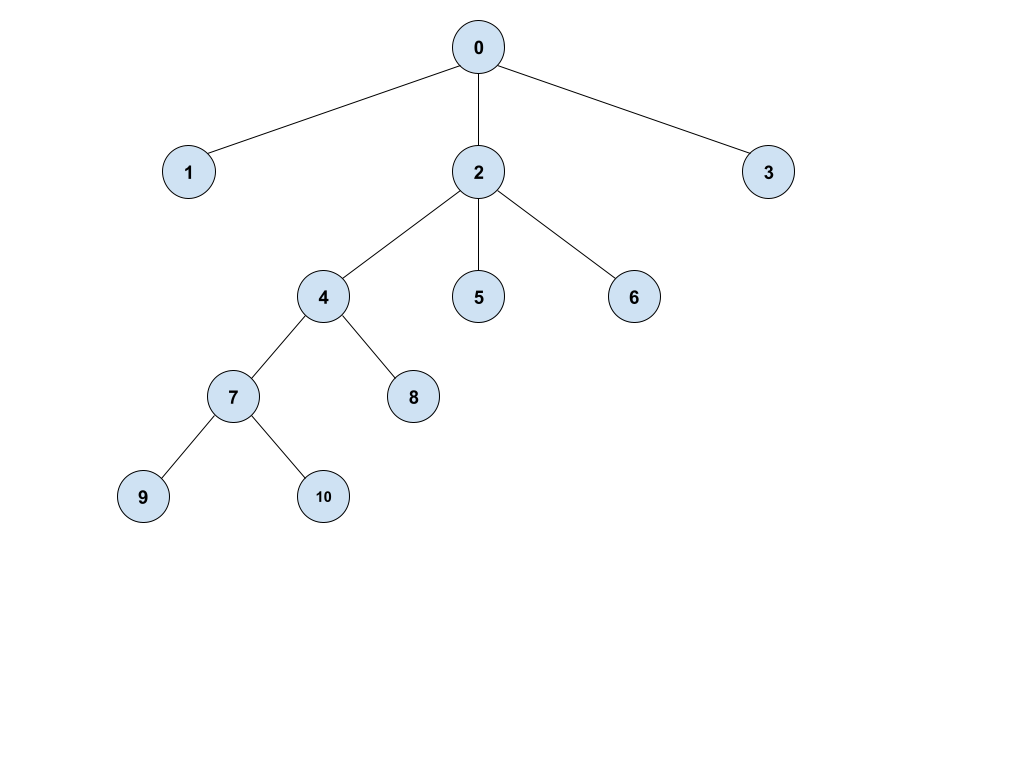
\includegraphics[width=0.9\linewidth]{images/LRMplanning.PNG}
        %     % \caption{} %% optional caption
            \label{fig:tree}
        \end{figure}

        \end{enumerate}

    \pagebreak
    %% End of Values %%%%%%%%%%%%%%%%%%%%%%%%%%%%%%%%%%%%%%%%%%%%%%%%%%%%%%



%%%%%%%%%%%%%%%%%%%%%%%%%%%%%%%%%%%%%%%%%%%%%%%%%%%%%%%%%%%%%%%%%%%%%%%%
    \subsection{Types}
    \label{sec:types}

    \pagebreak
    %% End of Values %%%%%%%%%%%%%%%%%%%%%%%%%%%%%%%%%%%%%%%%%%%%%%%%%%%%%%




%%%%%%%%%%%%%%%%%%%%%%%%%%%%%%%%%%%%%%%%%%%%%%%%%%%%%%%%%%%%%%%%%%%%%%%%
    \subsection{Definitions and Expressions}
    \label{sec:expr}

        \hspace{1cm}\begin{minipage}[h]{1\textwidth}
        \begin{grammar}
            % defn ::= Val
            <def> ::= \texttt{(}\ \texttt{val} \hyperref[subsec:id]{$ident$} $expr$ \texttt{)}\
            % defn ::= Expr
            \alt $expr$

            % expr ::= lit
            <expr> ::= $literal$
            % expr ::= var
            \alt \hyperref[subsec:id]{$ident$}
            % expr ::= unary
            \alt \hyperref[subsec:op]{\emph{unary-operator}} $expr$
            % expr ::= bin
            \alt \texttt{(}\ \hyperref[subsec:op]{\emph{binary-operator}} $expr$ $expr$ \texttt{)}
            % expr ::= Application
            \alt \texttt{(}\ \hyperref[subsec:id]{$ident$} \big\{\emph{expr}\big\} \texttt{)}
            % expr ::= let
            \alt \texttt{(}\ \texttt{let} \texttt{(}\  \texttt{[}\hyperref[subsec:id]{$ident$} $expr$\texttt{]}  \big\{\texttt{[}\hyperref[subsec:id]{$ident$} $expr$\texttt{]}\big\} \texttt{)}\ $expr$  \texttt{)}
            % expr ::= if
            \alt \texttt{(}\ \texttt{if} $expr$ $expr$ $expr$ \texttt{)}
            % expr ::= lambda
            \alt \texttt{(}\ \texttt{lambda} (\ \big\{$arguments$\big\} )\ $expr$ \texttt{)}

            <literal> ::=  \hyperref[subsec:intlit]{\emph{integer-literal}} |  \hyperref[subsec:boollit]{\emph{boolean-literal}} | \hyperref[subsec:charlit]{\emph{character}} | \hyperref[subsec:key]{leaf}

            <arguments> ::= $\epsilon$
            \alt \hyperref[subsec:id]{$ident$} :: $arguments$
            

        \end{grammar}
        \end{minipage}

        Expressions are values or parenthetical expressions.

        \subsubsection{Values}
        see \hyperref[sec:values]{Values}.


        


        \subsubsection{Parenthetical expressions} Parenthetical expressions are always withing parentheses and include function application, lambda expressions, global and local definitions, binary and unary operations, and if-statements. In the above concrete syntax, the parentheses in this font, \texttt{( ... )}, are syntax requirements, rather than denoting a grouping which is given by ( ... )

        \subsubsection{Function application}
        Function application in (g)ROOT always returns a value, and is written as the function \texttt{ID} followed by a list of zero or more expressions, which are its arguments. The arguments are not separated from the ID by parentheses. (g)ROOT has first-class functions, therefore functions can be passed as arguments. Currying is allowed.

        Example:

\cbcolor{dkgreen}
\cbstart
\begin{lstlisting}
(foo)
(bar a b)
((baz x) y)
\end{lstlisting}
\cbend

        \subsubsection{Lambda Expression}
        Lambda expressions are accomplished with the \texttt{lambda} keyword, a parentheses-enclosed list of 0 or more identifiers as formal arguments, followed by the expression that may use those arguments and/or any free variables. Nesting of lambda expressions is not allowed.

        Example:

\cbcolor{dkgreen}
\cbstart
\begin{lstlisting}
(lambda () #t)
(lambda (x) x)
(lambda (x y) (+ x y))

(lambda (a) (add2 a b))
\end{lstlisting}
\cbend

        \subsubsection{Global definitions} Global definitions are accomplished using the \texttt{val} keyword, followed by an identifier, followed by the expression which is to be bound to that value.

        Example:

\cbcolor{dkgreen}
\cbstart
\begin{lstlisting}
(val x 4)
(val y (+ x 5))
(val foo (lambda (arg) ( * arg arg)))
\end{lstlisting}
\cbend

        Calling a global definition with a preexisting identifier will re-bind that identifier to the new value - onlys allowed at the top level, and new definition must always of the same type as the previous definition.

        \subsubsection{Local definitions} Local definitions are found with the \texttt{let} expressions, which is the \texttt{let} keyword followed by the identifier(s) and the expression(s) to be bound to it, followed by the expression that local variable may be used. Let expressions must have at least one local binding. 

        Example:

\cbcolor{dkgreen}
\cbstart
\begin{lstlisting}
(let ([x 4]) (+ 2 x))    (; return 6 ;) 
(let ([x 4]) x)          (; return 4 ;) 
(let () y)               (; not allowed! ;)
\end{lstlisting}
\cbend

        Variables defined within the let binding are not defined outside of it, while variables globally relative to the let can be accessed within it. Since let bindings are a type of expression, this allows for chained let bindings.  

        Example:

\cbcolor{dkgreen}
\cbstart
\begin{lstlisting}
(let x 4 
    (let y 5 
        (let z 9 
            (+ x (- y z)))))
\end{lstlisting}
\cbend

        \subsubsection{If-expression}
        If-expressions are the only form of control flow in (g)ROOT, and are always formed with the \texttt{if} keyword followed by three expressions (the \emph{condition}, the \emph{true case} and the \emph{false case}). Omission of the false case is a syntax error, and the expressions are not separated by parentheses, brackets, or keywords.
        
        Example:

\cbcolor{dkgreen}
\cbstart
\begin{lstlisting}
(if #t 1 2)
(if (< 3 4) 
    (+ x y) 
    (- x y))
\end{lstlisting}
\cbend

        \subsubsection{Unary operators} Unary operations (used for boolean or signed negation) must not be enclosed in parentheses. They are accomplished with a unary operator in front of the expression they negate.

        Example:

\cbcolor{dkgreen}
\cbstart
\begin{lstlisting}
-3
-(+ 3 4)
-(if #t 2 3)
-x

!#t
!x
!(expr)
\end{lstlisting}
\cbend

        \subsubsection{Binary operators} The general use of binary operators is as follows: (\ \hyperref[subsec:op]{\emph{binary-operator}} $expr_1$ $expr_2$)

        The \textbf{arithmetic operators} (\ \texttt{+\ ,\ -\ ,\ *\ ,\ /\ ,\ mod }) take two expressions that evaluate to \hyperref[sec:values]{integers}. 

        The \textbf{comparator operators} (\ \texttt{==\ ,\ \textless\ ,\ \textgreater\ ,\ $\leq$ ,\ $\geq$\ ,\ != }) take two expressions that both evaluate to either \hyperref[sec:values]{integers} or \hyperref[sec:values]{booleans}.

        The \textbf{boolean operators} (\ \texttt{\&\& ,\ \textcolor{red}{||} }) take two expressions that evaluate to \hyperref[sec:values]{booleans}.





\pagebreak
%% End of Expressions %%%%%%%%%%%%%%%%%%%%%%%%%%%%%%%%%%%%%%%%%%%


    %%%%%%%%%%%%%%%%%%%%%%%%%%%%%%%%%%%%%%%%%%%%%%%%%%%%%%%%%%%%%%%%%%%%%%%%
    \subsection{Functions}
    \label{sec:func}

        \subsubsection{Built-In Functions}
        \textbf{Note}: Throughout this section, the character pair \texttt{tr} is used as shorthand to represent a tree value, an identifier bound to a tree value.

        There are four built-in functions which are integral to the tree data type. It is a checked-runtime error to call \texttt{elm, sib, cld} on a \texttt{leaf}:
        \begin{enumerate}
            \item \texttt{elm}

            Usage: \texttt{(elm tr)}

            Purpose: returns the element of the provided tree value \texttt{(tr)}

            \item \texttt{sib}

            Usage: \texttt{(sib tr)}

            Purpose: returns the sibling tree of the provided tree value \texttt{(tr)}

            \item \texttt{cld}

            Usage: \texttt{(cld tr)}

            Purpose: returns the child tree of the provided tree value \texttt{(tr)}

            \item \texttt{leaf?}
            
            Usage: \texttt{(leaf? tr)}

            Purpose: Returns boolean val \texttt{\#t} iff \texttt{tr} is a leaf.

            \item \texttt{tree}

            Usage: \texttt{(tree ELEMENT SIBLING CHILD)}

            Purpose: constructs a tree value containing the value ELEMENT, with sibling SIBLING and child CHILD
        \end{enumerate}

        \subsubsection{Standard Library Functions}
        \textbf{Note}: Throughout this section, the character pair \texttt{tr} is used as shorthand to represent a tree value, an identifier bound to a tree value.

        The first set of functions introduced in the standard library allow for programmers to use some of their beloved list functions present in other languages:
        \begin{enumerate}
            \item \texttt{(cons a b)}
            
            Creates a 1-ary tree approximating the functionality of single-dimensional list in other functional languages. \texttt{a} is any value not a tree, \texttt{b} may be \texttt{leaf} or \texttt{nil}.

            \item \texttt{(car tr)}
            
            Extracts the first value in the pair.

            \item \texttt{(cdr tr)}
            
            Extracts the second value in the pair.

            \item \texttt{(null? tr)}
            
            A predicate function that evaluates to true iff the pseudo-list is empty.

            \item \texttt{(val nil leaf)}
            
            A value \texttt{nil} that mirrors the built-in keyword leaf.

            \item \texttt{(append xs ys)}
            
            Append the list of elements in \texttt{ys} to the end of \texttt{xs}.

            \item \texttt{(revapp xs ys)}
            
            Append the list of elements in \texttt{ys} to the reverse of \texttt{xs}.

            
        \end{enumerate}

        Now some useful tree functions!
        \begin{enumerate}
            \item \texttt{(graft oak fir)}
            
            Appends a sibling tree \texttt{fir} to some other tree \texttt{oak}. The result of calling this function is a new tree in which \texttt{fir} is the rightmost sibling of \texttt{oak}. This function is extremely useful when re-shaping trees.

            \item \texttt{(level-flatten tr)} 
            
            Flattens the provided tree to a 1-ary tree, arranging elements in level-order.

            \item \texttt{(pre-flatten tr)}
            
            Flattens the provided tree to a 1-ary tree, arranging elements in pre-order.
            
            \item \texttt{(post-flatten tr)}
            
            Flattens the provided tree to a 1-ary tree, arranging elements in post-order.
            
            \item \texttt{(map f tr)}
            Maps a function \texttt{f} over every element of the provided tree \texttt{tr}.
            
            \item \texttt{(filter p? tr)}
            
            Constructs a new tree containing only elements that satisfy the predicate function \texttt{p?}, which must return a boolean value.
            
            \item \texttt{(level-fold fn base tr)}
            
            Folds a tree, visiting each element in a level-order traversal. Note that the accumulation function \texttt{fn} must take TWO arguments, the first of which is the current element, and second is the rest of the tree.
            
            \item \texttt{(pre-fold fn base tr)}
            
            Folds a tree, visiting each element in a pre-order traversal. Note that the accumulation function \texttt{fn} must take TWO arguments, the first of which is the current element, and second is the rest of the tree.

            \item \texttt{(post-fold fn base tr)}
            
            Folds a tree, visiting each element in a post-order traversal. Note that the accumulation function \texttt{fn} must take TWO arguments, the first of which is the current element, and second is the rest of the tree.
            
            \item \texttt{(fold fn base tr)}
            
            Folds a tree, in a more intuitively tree-like manner. Note that the accumulation function \texttt{fn} must take THREE arguments: the value of the current node, the sibling accumulator, and the child.accumulator.
            
            \item \texttt{(node-count tr)}
            
            Evaluates to the number of nodes in the provided tree.
            
            \item \texttt{(height tr)}
            
            Evaluates to the height of the provided tree.

        \end{enumerate}

        Higher-Order Functions:
        \begin{enumerate}
            \item \texttt{(curry f)}
            
            Allows for the partial application of a two-argument function.
            
            \item \texttt{(uncurry f)}
            
            Uncurries a previously curried function such that both of its arguments must be provided at the same time.
            
            \item \texttt{(o f g)}
            
            Given two single-argument functions, returns a single function which is the composition of \texttt{f} and \texttt{g}.
            
            \item \texttt{(flip f)}
            
            Given a two argument function, reverses the order in which the arguments are evaluated and passed to the function.
            
            \item \texttt{(flurry f)}
            
            Given a two argument function, reverses the order in which the arguments are evaluated and passed to the function, and allows for the partial application of that function. This function both flips and curries \texttt{f} (hence the fun name).

        \end{enumerate}

    \pagebreak
    %% End of Functions %%%%%%%%%%%%%%%%%%%%%%%%%%%%%%%%%%%%%%%%%%%


    %%%%%%%%%%%%%%%%%%%%%%%%%%%%%%%%%%%%%%%%%%%%%%%%%%%%%%%%%%%%%%%%%%%%%%%%
    \subsection{LRM Appendix}
    \label{sec:lrmapp}

\cbcolor{dkgreen}
\cbstart
\begin{lstlisting}
(; We can define standard list functions with our tree data type! Fun! ;)

(define (cons a b) (tree a leaf (tree b leaf leaf)))
(define (car   tr) (elm tr))
(define (cdr   tr) (cld tr))
(define (nil     ) leaf)
(define (null? tr) (leaf? tree))
   
(; a list function! ;)
(define append (xs ys)
    (if (null? xs)
        ys
        (cons (car xs) (append (cdr xs) ys))
    )
)
   
(; another list function! ;)
(define revapp (xs ys) ; (reverse xs) followed by ys
    (if (null? xs)
        ys
        (revapp (cdr xs) (cons (car xs) ys))
    )
)
   
(; appends a sibling tree (fir) to tree (oak) ;)
(define (graft oak fir)
    (if (leaf? oak)
        fir
        (tree (elm oak) (graft (sib oak) fir) (cld oak))
    )
)
   
(; attempt 4 
   this function flattens a tree, level-order ;)
(define (level-flatten tr)
    (if (leaf? tr)
        leaf
        (tree
            (elm tr)
            leaf
            (level-flatten (graft (sib tr) (cld tr)))
        )
    )
)
\end{lstlisting}
\cbend



flattening functions!

\cbcolor{dkgreen}
\cbstart
\begin{lstlisting}
(; this function flattens a tree, pre-order ;)
(define (pre-flatten tr)
    (if (leaf? tr)
        leaf
        (tree
            (elm tr)
            leaf
            (pre-flatten (graft (cld tr) (sib tr)))
        )
    )
)
   
   
(; this function flattens a tree, post-order ;)
(define (post-flatten tr)
    (if (leaf? tr)
        leaf
        (if (leaf? (cld tr))
            (tree
                (elm tr)
                leaf
                (post-flatten (sib tr)))
            (post-flatten (graft
                                (graft
                                    (cld tr)
                                    (tree (elm tr) leaf leaf))
                                (sib tr))
            )
        )
    )
)
\end{lstlisting}
\cbend


Let's create some higher order functions! Yay!

\cbcolor{dkgreen}
\cbstart
\begin{lstlisting}
(define (curry   f)   (lambda (x)   (lambda (y) (f x y))))
(define (uncurry f)   (lambda (x y) ((f x) y)))
(define (o       f g) (lambda (x)   (f (g x))))
(define (flip    f)   (lambda (x)   (lambda (y) (f y x))))


\end{lstlisting}
\cbend



function: (flurry func)
\begin{itemize}
    \item precondition:
    
    func is a function that takes exactly two args

    \item evalutation: 
    
    evaluates to a curried form of func, where:
        \begin{enumerate}
            \item the first value passed to the curried function is treated as the second argument to (func).
            \item the second value passed to the curried function is treated as the first argument to (func).
        \end{enumerate}

    \item note: flurry is a contraction of ``flip \& curry'', and we're very proud of the wordplay there.
\end{itemize}


\cbcolor{dkgreen}
\cbstart
\begin{lstlisting}
(define flurry (func)
    (curry (lambda (a b) (func b a)))
)


(; mapping function! ;)
(define (map f tr)
    (if (leaf? tr)
        leaf
        (tree
            (f (elm tr))
            (map f (sib tr))
            (map f (cld tr))
        )
    )
)
   

(; filter function! ;) 
(define filter (p? tr)
    (if (leaf? tr)
        leaf
        (if (p? (elm tr))
            (tree (elm tr) (filter p? (sib tr)) (filter p? (cld tr)))
            (filter p? (graft (cld tr) (sib tr)))
        )
    )
)
   
   
   

(; folding functions! ;) 

(; attempt 4 
   this function folds a tree, level-order ;) 
(define (level-fold fn base tr)
    (if (leaf? tr)
        base
        (fn
            (elm tr)
            (level-fold (graft (sib tr) (cld tr)))
        )
    )
)
   
(; this function folds a tree, pre-order ;) 
(define (pre-fold fn base tr)
    (if (leaf? tr)
        base
        (fn
            (elm tr)
            (pre-fold (graft (cld tr) (sib tr)))
        )
    )
)
   
(; this function folds a tree, post-order ;) 
(define (post-fold fn base tr)
    (if (leaf? tr)
        base
        (if (leaf? (cld tr))
            (fn (elm tr) (post-fold (sib tr)))
            (post-fold (graft
                            (graft (cld tr) (tree (elm tr) leaf leaf))
                                (sib tr)
                        )
            )
        )
    )
)
   
(; once we implement first-class functions, we 
   should find that the behaviors of these three
   functions are exactly equivalent to their
   lower-class cousins ;) 
(define (level-fold-flatten tr) (level-fold cons nil tr))
(define (pre-fold-flatten   tr) (pre-fold   cons nil tr))
(define (post-fold-flatten  tr) (post-fold  cons nil tr))

(; this function folds a tree, in a more intuitively 
   tree-like manner
   fn must take in three params: 
   - the current value   
   - the sibling accumulator
   - the child accumulator ;)     
(define (fold fn base tr)
    (if (leaf? tr)
        base
        (fn
            (elm tr)
            (fold fn base (sib tr))
            (fold fn base (cld tr))
        )
    )
)
   
   

(; some more fun folding functions! ;) 
(define (node-count tr)
    (pre-fold (lambda (elem count) (+ 1 count)) 0 tr)
)
   
(; this uses the tree fold to calculate the height! ;) 
(define (height tr)
    (fold
        (lambda (elem clds sibs) (+ 1 (max clds sibs)))
        0 tr
    )
)

(define (height-no-fold tr)
    (if (leaf? tr)
        0
        (max (height (sib tr)) 
            (+ 1 (height (cld tr)))
        )
    )
)
\end{lstlisting}
\cbend

    % \pagebreak
    %% End of LRM Appendix %%%%%%%%%%%%%%%%%%%%%%%%%%%%%%%%%%%%%%%%%%%

\pagebreak
%%%%%%%%%%%%%%%%%%%%%%%%%%%%%%%%%%%%%%%%%%%%%%%%%%%%%%%%%%%%%%%%%%%%%%%%%%%%%%%
%%%%%%%%%%%%%%%%%%%%%%%%%%%%%%%%%%%%%%%%%%%%%%%%%%%%%%%%%%%%%%%%%%%%%%%%%%%%%%%
%%%%%%%%%%%%%%%%%%%%%%%%%%%%%%%%%%% LRM %%%%%%%%%%%%%%%%%%%%%%%%%%%%%%%%%%%%%%%
%%%%%%%%%%%%%%%%%%%%%%%%%%%%%%%%%%%%%%%%%%%%%%%%%%%%%%%%%%%%%%%%%%%%%%%%%%%%%%%
%%%%%%%%%%%%%%%%%%%%%%%%%%%%%%%%%%%%%%%%%%%%%%%%%%%%%%%%%%%%%%%%%%%%%%%%%%%%%%%







%%%%%%%%%%%%%%%%%%%%%%%%%%%%%%%%%%%%%%%%%%%%%%%%%%%%%%%%%%%%%%%%%%%%%%%%%%%%%%%
%%%%%%%%%%%%%%%%%%%%%%%%%%%%%%%%%%%%%%%%%%%%%%%%%%%%%%%%%%%%%%%%%%%%%%%%%%%%%%%
%%%%%%%%%%%%%%%%%%%%%%%%%%%%%%%%%% PLAN %%%%%%%%%%%%%%%%%%%%%%%%%%%%%%%%%%%%%%%
%%%%%%%%%%%%%%%%%%%%%%%%%%%%%%%%%%%%%%%%%%%%%%%%%%%%%%%%%%%%%%%%%%%%%%%%%%%%%%%
%%%%%%%%%%%%%%%%%%%%%%%%%%%%%%%%%%%%%%%%%%%%%%%%%%%%%%%%%%%%%%%%%%%%%%%%%%%%%%%
\section{Project Plan}
\label{sec:PLAN}


    \pagebreak
    \subsection{Project Logs}

    \begin{figure}[h]
        \centering
        \fbox{\includegraphics[width=1\linewidth]{images/log\_dev.png}}
    \end{figure}


    \begin{figure}[h]
        \centering
        \begin{tabular}{cc}
            \begin{subfigure}{.5\textwidth}
                \centering
                \includegraphics[width=1\textwidth,height=3.8cm]{images/log\_amy.png}
                \label{fig:Amy}
            \end{subfigure} &
            \begin{subfigure}{.5\textwidth}
                \centering
                \includegraphics[width=1\textwidth,height=3.8cm]{images/log\_nik.png}
                \label{fig:Nik}
            \end{subfigure} \\ 
            \begin{subfigure}{.5\textwidth}
                \centering
                \includegraphics[width=1\textwidth,height=3.8cm]{images/log\_zach1.png}
                \label{fig:Zach}
            \end{subfigure} &
            \begin{subfigure}{.5\textwidth}
                \centering
                \includegraphics[width=1\textwidth,height=3.8cm]{images/log\_sam1.png}
                \label{fig:Zam}
            \end{subfigure} \\
            \begin{subfigure}{.5\textwidth}
                \centering
                \includegraphics[width=1\textwidth,height=3.8cm]{images/log\_eliza1.png}
                \label{fig:Eliza}
            \end{subfigure} &
        \end{tabular}
        % \label{fig:MULTI_NAME}
    \end{figure}


\pagebreak
%%%%%%%%%%%%%%%%%%%%%%%%%%%%%%%%%%%%%%%%%%%%%%%%%%%%%%%%%%%%%%%%%%%%%%%%%%%%%%%
%%%%%%%%%%%%%%%%%%%%%%%%%%%%%%%%%%%%%%%%%%%%%%%%%%%%%%%%%%%%%%%%%%%%%%%%%%%%%%%
%%%%%%%%%%%%%%%%%%%%%%%%%%%%%%%%%% PLAN %%%%%%%%%%%%%%%%%%%%%%%%%%%%%%%%%%%%%%%
%%%%%%%%%%%%%%%%%%%%%%%%%%%%%%%%%%%%%%%%%%%%%%%%%%%%%%%%%%%%%%%%%%%%%%%%%%%%%%%
%%%%%%%%%%%%%%%%%%%%%%%%%%%%%%%%%%%%%%%%%%%%%%%%%%%%%%%%%%%%%%%%%%%%%%%%%%%%%%%






%%%%%%%%%%%%%%%%%%%%%%%%%%%%%%%%%%%%%%%%%%%%%%%%%%%%%%%%%%%%%%%%%%%%%%%%%%%%%%%
%%%%%%%%%%%%%%%%%%%%%%%%%%%%%%%%%%%%%%%%%%%%%%%%%%%%%%%%%%%%%%%%%%%%%%%%%%%%%%%
%%%%%%%%%%%%%%%%%%%%%%%%%%%%%%%%% DESIGN %%%%%%%%%%%%%%%%%%%%%%%%%%%%%%%%%%%%%%
%%%%%%%%%%%%%%%%%%%%%%%%%%%%%%%%%%%%%%%%%%%%%%%%%%%%%%%%%%%%%%%%%%%%%%%%%%%%%%%
%%%%%%%%%%%%%%%%%%%%%%%%%%%%%%%%%%%%%%%%%%%%%%%%%%%%%%%%%%%%%%%%%%%%%%%%%%%%%%%
\section{Architectural Design}
\label{sec:DESIGN}

    \begin{figure}[h]
        \centering
        \fbox{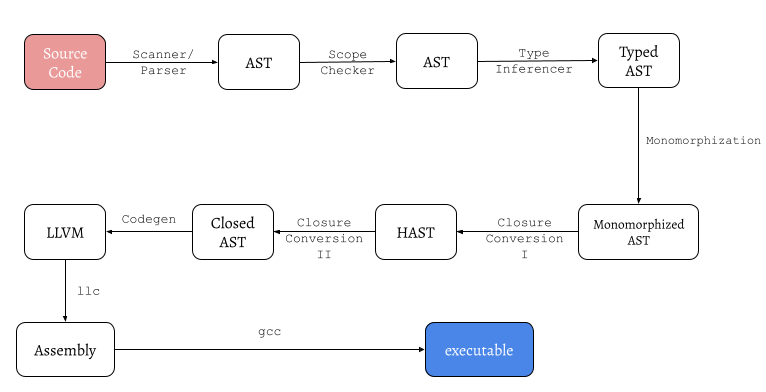
\includegraphics[width=1.1\linewidth]{images/phases.png}}
    \end{figure}
    

\pagebreak
%%%%%%%%%%%%%%%%%%%%%%%%%%%%%%%%%%%%%%%%%%%%%%%%%%%%%%%%%%%%%%%%%%%%%%%%%%%%%%%
%%%%%%%%%%%%%%%%%%%%%%%%%%%%%%%%%%%%%%%%%%%%%%%%%%%%%%%%%%%%%%%%%%%%%%%%%%%%%%%
%%%%%%%%%%%%%%%%%%%%%%%%%%%%%%%%% DESIGN %%%%%%%%%%%%%%%%%%%%%%%%%%%%%%%%%%%%%%
%%%%%%%%%%%%%%%%%%%%%%%%%%%%%%%%%%%%%%%%%%%%%%%%%%%%%%%%%%%%%%%%%%%%%%%%%%%%%%%
%%%%%%%%%%%%%%%%%%%%%%%%%%%%%%%%%%%%%%%%%%%%%%%%%%%%%%%%%%%%%%%%%%%%%%%%%%%%%%%











%%%%%%%%%%%%%%%%%%%%%%%%%%%%%%%%%%%%%%%%%%%%%%%%%%%%%%%%%%%%%%%%%%%%%%%%%%%%%%%
%%%%%%%%%%%%%%%%%%%%%%%%%%%%%%%%%%%%%%%%%%%%%%%%%%%%%%%%%%%%%%%%%%%%%%%%%%%%%%%
%%%%%%%%%%%%%%%%%%%%%%%%%%%%%%%%%% TEST %%%%%%%%%%%%%%%%%%%%%%%%%%%%%%%%%%%%%%%
%%%%%%%%%%%%%%%%%%%%%%%%%%%%%%%%%%%%%%%%%%%%%%%%%%%%%%%%%%%%%%%%%%%%%%%%%%%%%%%
%%%%%%%%%%%%%%%%%%%%%%%%%%%%%%%%%%%%%%%%%%%%%%%%%%%%%%%%%%%%%%%%%%%%%%%%%%%%%%%
\section{Test Plan}
\label{sec:TEST}

\pagebreak
%%%%%%%%%%%%%%%%%%%%%%%%%%%%%%%%%%%%%%%%%%%%%%%%%%%%%%%%%%%%%%%%%%%%%%%%%%%%%%%
%%%%%%%%%%%%%%%%%%%%%%%%%%%%%%%%%%%%%%%%%%%%%%%%%%%%%%%%%%%%%%%%%%%%%%%%%%%%%%%
%%%%%%%%%%%%%%%%%%%%%%%%%%%%%%%%%% TEST %%%%%%%%%%%%%%%%%%%%%%%%%%%%%%%%%%%%%%%
%%%%%%%%%%%%%%%%%%%%%%%%%%%%%%%%%%%%%%%%%%%%%%%%%%%%%%%%%%%%%%%%%%%%%%%%%%%%%%%
%%%%%%%%%%%%%%%%%%%%%%%%%%%%%%%%%%%%%%%%%%%%%%%%%%%%%%%%%%%%%%%%%%%%%%%%%%%%%%%





%%%%%%%%%%%%%%%%%%%%%%%%%%%%%%%%%%%%%%%%%%%%%%%%%%%%%%%%%%%%%%%%%%%%%%%%%%%%%%%
%%%%%%%%%%%%%%%%%%%%%%%%%%%%%%%%%%%%%%%%%%%%%%%%%%%%%%%%%%%%%%%%%%%%%%%%%%%%%%%
%%%%%%%%%%%%%%%%%%%%%%%%%%%%%%%% LESSON %%%%%%%%%%%%%%%%%%%%%%%%%%%%%%%%%%%%%%%
%%%%%%%%%%%%%%%%%%%%%%%%%%%%%%%%%%%%%%%%%%%%%%%%%%%%%%%%%%%%%%%%%%%%%%%%%%%%%%%
%%%%%%%%%%%%%%%%%%%%%%%%%%%%%%%%%%%%%%%%%%%%%%%%%%%%%%%%%%%%%%%%%%%%%%%%%%%%%%%
\section{Lessons Learned}
\label{sec:LESSON}

    \subsection*{Amy Bui}

    My main takeaway is that compiler writing, or even writing just a single optimization for a compiler, is a very complicated endeavor. We did not end up with a lot of our original goals and features we intended for our functional language, but the detours we took while exploring this whole other paradigm was very enriching, and I was never bored and always challenged. Everyone should write a compiler at least once before graduating. This was a great project in demonstrating the practical application of the concepts and theory we learnt in 170 and 105, and I'd recommend taking both classes before 107 or at the same time for a more comfortable time. I have a lot of appreciation for people who do research and contribute to the field of functional languages, and the complexity of lambda calculus. My advice to future students is that you should have a burning desire to implement type inferencing and lambda calculus before you settle on a a functional language as your project topic; I never knew how much we took static typing and statment blocks for granted. Or you can get a thrill from just taking on this challenge. 
    
    \subsection*{Nickolas Gravel}
        \begin{itemize}
            \item Takeaway:
            \item Advice: 
        \end{itemize}
    
    \subsection*{Sam Russo}
        \begin{itemize}
            \item Takeaway:
            \item Advice: 
        \end{itemize}
    
    \subsection*{Eliza Encherman}
        \begin{itemize}
            \item Takeaway:
            \item Advice: 
        \end{itemize}
    
    \subsection*{Zachary Goldstein}
        \begin{itemize}
            \item Takeaway:
            \item Advice: 
        \end{itemize}

\pagebreak
%%%%%%%%%%%%%%%%%%%%%%%%%%%%%%%%%%%%%%%%%%%%%%%%%%%%%%%%%%%%%%%%%%%%%%%%%%%%%%%
%%%%%%%%%%%%%%%%%%%%%%%%%%%%%%%%%%%%%%%%%%%%%%%%%%%%%%%%%%%%%%%%%%%%%%%%%%%%%%%
%%%%%%%%%%%%%%%%%%%%%%%%%%%%%%%%%% LESSON %%%%%%%%%%%%%%%%%%%%%%%%%%%%%%%%%%%%%
%%%%%%%%%%%%%%%%%%%%%%%%%%%%%%%%%%%%%%%%%%%%%%%%%%%%%%%%%%%%%%%%%%%%%%%%%%%%%%%
%%%%%%%%%%%%%%%%%%%%%%%%%%%%%%%%%%%%%%%%%%%%%%%%%%%%%%%%%%%%%%%%%%%%%%%%%%%%%%%







%%%%%%%%%%%%%%%%%%%%%%%%%%%%%%%%%%%%%%%%%%%%%%%%%%%%%%%%%%%%%%%%%%%%%%%%%%%%%%%
%%%%%%%%%%%%%%%%%%%%%%%%%%%%%%%%%%%%%%%%%%%%%%%%%%%%%%%%%%%%%%%%%%%%%%%%%%%%%%%
%%%%%%%%%%%%%%%%%%%%%%%%%%%%%%%%%% APPENDIX %%%%%%%%%%%%%%%%%%%%%%%%%%%%%%%%%%%
%%%%%%%%%%%%%%%%%%%%%%%%%%%%%%%%%%%%%%%%%%%%%%%%%%%%%%%%%%%%%%%%%%%%%%%%%%%%%%%
%%%%%%%%%%%%%%%%%%%%%%%%%%%%%%%%%%%%%%%%%%%%%%%%%%%%%%%%%%%%%%%%%%%%%%%%%%%%%%%
\section{Appendix}
\label{sec:APPENDIX}

    \subsection{\texttt{ast.ml}}
    \label{app:ast}
    Author(s): Sam, Eliza, Amy, Nik, Zach
\begin{lstlisting}
(* Abstract Syntax Tree (AST) for Groot *)
(* Type of Variable Names *)
type ident = string

type expr =
  | Literal of value
  | Var     of ident
  | If      of expr * expr * expr
  | Apply   of expr * expr list
  | Let     of (ident * expr) list * expr
  | Lambda  of ident list * expr
and value =
  |Char    of char
  | Int     of int
  | Bool    of bool
  | Root    of tree
and tree =
  |Leaf
  | Branch of expr * tree * tree

type defn =
  | Val of ident * expr
  | Expr of expr

type prog = defn list


(* Pretty printing functions *)
(* toString for Ast.expr *)
let rec string_of_expr = function
  | Literal(lit) -> string_of_value lit
  | Var(v) -> v
  | If(condition, true_branch, false_branch) ->
    "(if "  ^ string_of_expr condition ^ " "
    ^ string_of_expr true_branch ^ " "
    ^ string_of_expr false_branch ^ ")"
  | Apply(f, args) ->
    "(" ^ string_of_expr f ^ " "
    ^ String.concat " " (List.map string_of_expr args) ^ ")"
  | Let(binds, body)   ->
    let string_of_binding = function
        (id, e) -> "[" ^ id ^ " " ^ (string_of_expr e) ^ "]"
    in
    "(let (" ^ String.concat " " (List.map string_of_binding binds) ^ ") "
    ^ string_of_expr body ^ ")"
  | Lambda(formals, body) ->
    "(lambda (" ^ String.concat " " formals ^ ") "
    ^ string_of_expr body ^ ")"

(* toString for Ast.value *)
and string_of_value = function
  | Char(c)     -> "'" ^ String.make 1 c ^ "'"
  | Int(i)      -> string_of_int i
  | Bool(b)     -> if b then "#t" else "#f"
  | Root(tr)    -> string_of_tree tr

(* toString for Ast.tree *)
and string_of_tree = function
  | Leaf -> "leaf"
  | Branch(ex, sib, child) ->
    (* Branch type is given by "tree" string *)
    "(tree " ^ string_of_expr ex ^ " "
    ^ string_of_tree sib ^ " "
    ^ string_of_tree child ^ ")"

(* toString for Ast.defn *)
let string_of_defn = function
  | Val(id, e) -> "(val " ^ id ^ " " ^ string_of_expr e ^ ")"
  | Expr(e)    -> string_of_expr e

(* toString for Ast.prog *)
let string_of_prog defns =
    String.concat "\n" (List.map string_of_defn defns) ^ "\n"  
\end{lstlisting}
\pagebreak


    \subsection{\texttt{scanner.mll}}
    \label{app:scanner}
    Author(s): Sam, Eliza, Amy, Nik, Zach
\begin{lstlisting}
(* Header *)
{ open Parser }

(* Regular Expressions *)
let digit = ['0'-'9']
let integer = ['-']?['0'-'9']+
let alpha = ['a'-'z']
let leaf = ("leaf"|"()")
let chrcode = digit+

(* all visible characters, excluding ()'[]\;{}| *)
let ident = ['!'-'&' '*'-':' '<'-'Z' '`'-'z' '~' '|']
            ['!'-'&' '*'-':' '<'-'Z' '^'-'z' '~' '|']*


(* ToKeNiZe *)
rule tokenize = parse
  | [' ' '\n' '\t' '\r'] { tokenize lexbuf }
  | "(;"                 { comment lexbuf }
  | '('                  { LPAREN }
  | ')'                  { RPAREN }
  | '['                  { LSQUARE }
  | ']'                  { RSQUARE }
  | "tree"               { BRANCH }
  | "leaf"               { LEAF }
  | "if"                 { IF }
  | "'"                  { apos_handler lexbuf }
  | integer as ival      { INT(int_of_string ival) }
  | "#t"                 { BOOL(true) }
  | "#f"                 { BOOL(false) }
  | "lambda"             { LAMBDA }
  | "let"                { LET }
  | "val"                { VAL }
  | ident as id          { ID(id) }
  | eof                  { EOF }
  | _                    { Diagnostic.error
                            (Diagnostic.lex_error "unrecognized character" 
                            lexbuf) }
and comment = parse
  | ";)"                 { tokenize lexbuf }
  | _                    { comment lexbuf }

(* apostrophe handler *)
and apos_handler = parse
  | '('[^''']      { tree_builder lexbuf }
  | '''            { Diagnostic.error
                    (Diagnostic.lex_error "empty character literal" lexbuf) }
  | '\\'           { escaped_char_handler lexbuf }
  | _ as c         { char_builder c lexbuf }

and tree_builder = parse
  | _ { Diagnostic.error(Diagnostic.Unimplemented "in-place tree syntax") }

and char_builder c = parse
  | '''   { CHAR(c) }
  | _ { Diagnostic.error
          (Diagnostic.lex_error ("character literal contains more " 
           ^ "than one token") lexbuf) }

and escaped_char_handler = parse
  | '\\' { char_builder '\\' lexbuf }
  | '"'  { char_builder '\"' lexbuf  }
  | '''  { char_builder '\'' lexbuf  }
  | 'n'  { char_builder '\n' lexbuf  }
  | 'r'  { char_builder '\r' lexbuf  }
  | 't'  { char_builder '\t' lexbuf  }
  | 'b'  { char_builder '\b' lexbuf  }
  | ' '  { char_builder '\ ' lexbuf  }
  | chrcode as ord
         { print_string ord; if int_of_string ord > 255
           then Diagnostic.error
                (Diagnostic.lex_error "invalid escape sequence ASCII value" 
                lexbuf)
           else char_builder (Char.chr (int_of_string ord)) lexbuf }
  | _    { Diagnostic.error
          (Diagnostic.lex_error "unrecognized escape sequence" lexbuf) }
\end{lstlisting}
    \pagebreak


    \subsection{\texttt{parser.mly}}
    \label{app:parser}
    Author(s): Sam, Eliza, Amy, Nik, Zach
\begin{lstlisting}
/* Header */
%{ open Ast %}

/* Tokens */
%token LPAREN  RPAREN
%token LSQUARE RSQUARE
%token PLUS MINUS TIMES DIVIDE MOD
%token EQ NEQ LT GT LEQ GEQ AND OR NOT
%token IF
%token <char> CHAR
%token <int>  INT
%token <bool> BOOL
%token <string> ID
%token BRANCH LEAF
%token EOF
%token LAMBDA LET VAL

/* Precedence */
%nonassoc OR
%nonassoc AND
%nonassoc LT GT
%nonassoc EQ NEQ
%nonassoc LEQ GEQ
%nonassoc PLUS MINUS
%nonassoc TIMES DIVIDE
%nonassoc NEG
%nonassoc NOT
%nonassoc BRANCH LEAF


/* Declarations */
%start prog
%type <Ast.prog> prog

%%

prog:
  | defn_list EOF                 { $1 }

defn_list:
  | /* nothing */                 { [] }
  | defn defn_list                { $1 :: $2 }

defn:
  | expr                          { Expr($1) }
  | LPAREN VAL ID expr RPAREN     { Val($3, $4) }

formals_opt:
  | /* nothing */                 { [] }
  | formal_list                   { $1 }

formal_list:
  | ID                            { [$1] }
  | ID formal_list                { $1 :: $2 }


/* Rules */
value:
  | CHAR                          { Char($1) }
  | INT                           { Int($1) }
  | BOOL                          { Bool($1) }
  | tree                          { Root($1) }
  /* ! Note: tree is not a token - no need for a ROOT token while scanning */


tree:
  | LEAF                                  { Leaf }
  | LPAREN BRANCH expr tree tree RPAREN   { Branch($3, $4, $5) }


let_binding_list:
  | /* nothing */                             { [] }
  | LSQUARE RSQUARE let_binding_list  
    { Diagnostic.warning (Diagnostic.parse_warning "empty let binding" 1); $3 } 
    /* NON FATAL */
  | LSQUARE expr RSQUARE let_binding_list     
    { Diagnostic.error (Diagnostic.parse_error ("let binding must contain" 
      ^ " id and value") 2) } /* FATAL */
  | LSQUARE ID expr RSQUARE let_binding_list  { ($2, $3) :: $5 }


expr_list:
  | /* null */         { [] }
  | expr expr_list     { $1 :: $2 }


expr:
  | value                                                 { Literal($1) }
  | ID                                                    { Var($1) }
  | LPAREN expr expr_list RPAREN                          { Apply($2, $3) }
  | LPAREN LET LPAREN let_binding_list RPAREN expr RPAREN { Let($4, $6)}
  | LPAREN IF expr expr expr RPAREN                       { If($3, $4, $5) }
  | LPAREN LAMBDA LPAREN formals_opt RPAREN expr RPAREN   { Lambda($4, $6) }
\end{lstlisting}
    \pagebreak


    \subsection{\texttt{scope.ml}}
    \label{app:scope}
    Author(s): Amy, Eliza
\begin{lstlisting}
(* Name (scope) checks variable names *)
open Ast

(* toplevel naming environment, preloaded with built-ins *)
let nameEnv = List.fold_right List.cons [ "printi"; "printb"; "printc";
                                            "+"; "-"; "*"; "/"; "mod";
                                            "<"; ">"; ">="; "<="; "~";
                                            "!=i"; "=i"; "&&"; "||"; "not"  ] []

(* Takes and AST and checks if variables are bound in scope.
    Returns same AST if so, otherwise raises Unbound variable error
    if a variable is unbound. *)
let check defns =

  (* Recursively checks the scope of variables names used in an expression *)
  let rec checkExpr expression rho =
    let rec exp e = match e with
        Literal _ -> ()
      | Var id -> 
          if List.mem id rho then ()
          else Diagnostic.error (Diagnostic.Unbound id)
      | If (e1, e2, e3) ->
          let (_, _, _) = (exp e1, exp e2, exp e3) in ()
      | Apply (f, args) ->
          let _ = exp f in List.iter exp args
      | Let (bs, body) ->
          let (xs, es) = List.split bs in
          let () = List.iter exp es in
          checkExpr body (List.fold_right List.cons xs rho)
      | Lambda (formals, body) ->
          checkExpr body (List.fold_right List.cons formals rho)
    in exp expression
  in

  let rec checkDef ds env =
    match ds with
      [] -> env
    | f :: rest ->
      let env' =
        (match f with
            Val (id, exp) ->
            let () = checkExpr exp env in
            id :: env
          | Expr exp -> let () = checkExpr exp env in env)
      in checkDef rest env'
  in
  let _ = checkDef defns nameEnv in

  (* Returns the AST if no error raised *)
  defns
\end{lstlisting}
    \pagebreak



    \subsection{\texttt{tast.ml}}
    \label{app:tast}
    Author(s): Sam, Nik
\begin{lstlisting}
(* TAST -- Type inference. *)

open Ast

exception Type_error of string
let type_error msg = raise (Type_error msg)

type gtype =
  | TYCON of tycon
  | TYVAR of tyvar
  | CONAPP of conapp
and tycon =
  | TyInt
  | TyBool
  | TyChar
  | TArrow of gtype
and tyvar =
  | TVariable of int
and conapp = (tycon * gtype list)

type tyscheme = tyvar list * gtype

let inttype = TYCON TyInt
let chartype = TYCON TyChar
let booltype = TYCON TyBool
let functiontype resultType formalsTypes =
      CONAPP (TArrow resultType, formalsTypes)


(* TAST expression *)
type texpr = gtype * tx
and tx =
  | TLiteral     of tvalue
  | TypedVar     of ident
  | TypedIf      of texpr * texpr * texpr
  | TypedApply   of texpr * texpr list
  | TypedLet     of (ident * texpr) list * texpr
  | TypedLambda  of (gtype * ident) list * texpr
and tvalue = TChar of char | TInt of int | TBool of bool | TRoot of ttree
and ttree = TLeaf | TBranch of tvalue * ttree * ttree

type tdefn = TVal of ident * texpr | TExpr of texpr
type tprog = tdefn list

(* Pretty printer *)

(* String of gtypes *)
let rec string_of_ttype = function
  | TYCON ty -> string_of_tycon ty
  | TYVAR tp -> string_of_tyvar tp
  | CONAPP con -> string_of_conapp con
and string_of_tycon = function
  | TyInt -> "int"
  | TyBool -> "bool"
  | TyChar -> "char"
  | TArrow (retty) -> string_of_ttype retty
and string_of_tyvar = function
  | TVariable n -> "'" ^ string_of_int n
and string_of_conapp (tyc, tys) =
string_of_tycon tyc ^ " (" 
    ^ String.concat " " (List.map string_of_ttype tys) ^ ")"

and string_of_subs = function
  | [] -> ""
  | (t1, t2) :: cs ->
      "(" ^ string_of_tyvar t1 ^ ", " ^ string_of_ttype t2 ^ ") "
      ^ string_of_subs cs

and string_of_context = function
  | [] -> ""
  | (ident, (tvs, gt)) :: ctx ->
      "\n=: " ^ ident ^ ", (["
      ^ String.concat ", " (List.map string_of_tyvar tvs)
      ^ "], " ^ string_of_ttype gt ^ ")" ^ string_of_context ctx

and string_of_tyformals (gt, ident) =
    "(" ^ ident ^ " : " ^ string_of_ttype gt ^ ")"

(* String of a typed expression (texpr) == (type, t-expression) *)
let rec string_of_texpr (typ, exp) =
    "[" ^ string_of_ttype typ ^ "] " ^ string_of_tx exp
and string_of_tx = function
    TLiteral v -> string_of_tvalue v
  | TypedVar id -> id
  | TypedIf (te1, te2, te3) ->
    "(if "  ^ string_of_texpr te1 ^ " "
    ^ string_of_texpr te2 ^ " "
    ^ string_of_texpr te3 ^ ")"
  | TypedApply (f, args) ->
    "(" ^ string_of_texpr f ^ " "
    ^ String.concat " " (List.map string_of_texpr args) ^ ")"
  | TypedLet (binds, body) ->
    let string_of_binding (id, e) =
      "[" ^ id ^ " " ^ (string_of_texpr e) ^ "]"
    in
    "(let ("  ^ String.concat " " (List.map string_of_binding binds) ^ ") "
    ^ string_of_texpr body ^ ")"
  | TypedLambda (formals, body) ->
    let formalStringlist = List.map (fun (ty, x) ->
        string_of_ttype ty ^ " " ^ x) formals in
    "(lambda (" ^ String.concat ", "  formalStringlist
    ^ ") " ^ string_of_texpr body ^ ")"

(* toString for Sast.svalue *)
and string_of_tvalue = function
  | TChar c -> String.make 1 c
  | TInt i -> string_of_int i
  | TBool b -> if b then "#t" else "#f"
  | TRoot tr -> string_of_ttree tr

(* toString for Sast.stree *)
and string_of_ttree = function
    TLeaf -> "leaf"
  | TBranch (v, sib, child) ->
    "(tree " ^ string_of_tvalue v ^ " "
    ^ string_of_ttree sib ^ " "
    ^ string_of_ttree child ^ ")"


(* String of a typed defn (tdefn) *)
let string_of_tdefn = function
  | TVal (id, te) -> "(val " ^ id ^ " " ^ string_of_texpr te ^ ")"
  | TExpr te    -> string_of_texpr te


(* String of the tprog == tdefn list *)
let string_of_tprog tdefns =
String.concat "\n" (List.map string_of_tdefn tdefns) ^ "\n"
\end{lstlisting}
    \pagebreak


    \subsection{\texttt{infer.ml}}
    \label{app:infer}
    Author(s): Sam, Eliza, Nik
\begin{lstlisting}
open Ast
open Tast
module StringMap = Map.Make (String)

(* prims - initializes context with built-in functions with their types *)
(* prims : (id * tyvar) list * (tycon * gtype list) *)
let prims =
  [
    ("printb",  ([ TVariable (-1) ], Tast.functiontype inttype [ booltype ]));
    ("printi",  ([ TVariable (-2) ], Tast.functiontype inttype [ inttype ]));
    ("printc",  ([ TVariable (-3) ], Tast.functiontype inttype [ chartype ]));
    ("+",       ([ TVariable (-4) ], Tast.functiontype inttype [ inttype; inttype ]));
    ("-",       ([ TVariable (-4) ], Tast.functiontype inttype [ inttype; inttype ]));
    ("/",       ([ TVariable (-4) ], Tast.functiontype inttype [ inttype; inttype ]));
    ("*",       ([ TVariable (-4) ], Tast.functiontype inttype [ inttype; inttype ]));
    ("mod",     ([ TVariable (-4) ], Tast.functiontype inttype [ inttype; inttype ]));
    ("<",       ([ TVariable (-5) ], Tast.functiontype booltype [ inttype; inttype ]));
    (">",       ([ TVariable (-5) ], Tast.functiontype booltype [ inttype; inttype ]));
    ("<=",      ([ TVariable (-5) ], Tast.functiontype booltype [ inttype; inttype ]));
    (">=",      ([ TVariable (-5) ], Tast.functiontype booltype [ inttype; inttype ]));
    ("=i",      ([ TVariable (-5) ], Tast.functiontype booltype [ inttype; inttype ]));
    ( "!=i",    ([ TVariable (-5) ], Tast.functiontype booltype [ inttype; inttype ]) );
    ( "&&",     ([ TVariable (-6) ], Tast.functiontype booltype [ booltype; booltype ]) );
    ( "||",     ([ TVariable (-6) ], Tast.functiontype booltype [ booltype; booltype ]) );
    ("not",     ([ TVariable (-7) ], Tast.functiontype booltype [ booltype ]));
    ("~",       ([TVariable (-2)], Tast.functiontype inttype [inttype]))
  ]

(* is_ftv - returns true if 'gt' is equal to free type variable 'var'
    (i.e. 'gt' is a type variable and 'var' is a free type variable). For the
    conapp case, we recurse over the conapp's gtype list searching for any free
    type variables. When this function returns true it means the type variable
    is matching *)
let rec is_ftv (var : tyvar) (gt : gtype) =
  match gt with
  | TYCON _ -> false
  | TYVAR v -> v = var
  | CONAPP (_, gtlst) ->
    (* if any x in gtlst is ftv this returns true, else returns false *)
    List.fold_left (fun acc x -> is_ftv var x || acc) false gtlst

(* ftvs - returns a list of free type variables amongst a collection 
   of gtypes *)
(* retty : tyvar list *)
let rec ftvs (ty : gtype) =
  match ty with
  | TYVAR t -> [ t ]
  | TYCON _ -> []
  | CONAPP (_, gtlst) -> List.fold_left (fun acc x -> acc @ ftvs x) [] gtlst

(* fresh - returns a fresh gtype variable (integer) *)
let fresh =
  let k = ref 0 in
  (* fun () -> incr k; TVariable !k *)
  fun () -> incr k; TYVAR (TVariable !k)


(* sub - updates a list of constraints with substitutions in theta *)
let sub (theta : (tyvar * gtype) list) (cns : (gtype * gtype) list) =
  (* sub_one - takes in single constraint and updates it with substitution in theta *)
  let sub_one (cn : gtype * gtype) =
    List.fold_left
      (fun ((c1, c2) : gtype * gtype) ((tv, gt) : tyvar * gtype) ->
          match (c1, c2) with
          | TYVAR t1, TYVAR t2 ->
            if tv = t1 then (gt, c2) else if tv = t2 then (c1, gt) else (c1, c2)
          | TYVAR t1, _ -> if tv = t1 then (gt, c2) else (c1, c2)
          | _, TYVAR t2 -> if tv = t2 then (c1, gt) else (c1, c2)
          | _, _ -> (c1, c2))
      cn theta
  in
  List.map sub_one cns

(* compose - applies the substitutions in theta1 to theta2 *)
let compose theta1 theta2 =
  (* sub_one - takes a single substitution in theta1 and applies it to theta2 *)
  let sub_one cn =
    List.fold_left
      (fun (acc : tyvar * gtype) (one_sub : tyvar * gtype) ->
          match (acc, one_sub) with
          | (a1, TYVAR a2), (s1, TYVAR s2) ->
            if s1 = a1 then (s1, TYVAR a2)
            else if s1 = a2 then (a1, TYVAR s2)
            else acc
          | (a1, a2), (s1, TYVAR _) -> if a1 = s1 then (s1, a2) else acc
          | (a1, _), (s1, s2) -> if a1 = s1 then (s1, s2) else acc)
      cn theta1
  in
  List.map sub_one theta2

(* solve': solves a single constraint 'c' *)
let rec solve' (c : gtype * gtype) =
  match c with
  | TYVAR t1, TYVAR t2 -> [ (t1, TYVAR t2) ]
  | TYVAR t1, TYCON t2 -> [ (t1, TYCON t2) ]
  | TYVAR t1, CONAPP t2 ->
    if is_ftv t1 (CONAPP t2) then
      Diagnostic.error (Diagnostic.TypeError "type variable is not free type in type constructor")
    else [ (t1, CONAPP t2) ]
  | TYCON t1, TYVAR t2 -> solve' (TYVAR t2, TYCON t1)
  | TYCON (TArrow (TYVAR t1)), TYCON t2 -> [ (t1, TYCON t2) ]
  | TYCON t1, TYCON (TArrow (TYVAR t2)) -> [ (t2, TYCON t1) ]
  | TYCON t1, TYCON t2 ->
    if t1 = t2 then []
    else
      Diagnostic.error (Diagnostic.TypeError
        ("type constructor mismatch " ^ string_of_tycon t1
          ^ " != " ^ string_of_tycon t2))
  | TYCON t1, CONAPP t2 ->
    Diagnostic.error (Diagnostic.TypeError
      ("type constructor mismatch " ^ string_of_tycon t1
      ^ " != " ^ string_of_conapp t2))
  | CONAPP t1, TYVAR t2 -> solve' (TYVAR t2, CONAPP t1)
  | CONAPP t1, TYCON t2 ->
    Diagnostic.error (Diagnostic.TypeError
      ("type constructor mismatch " ^ string_of_conapp t1
        ^ " != " ^ string_of_tycon t2))
  | CONAPP t1, CONAPP t2 -> (
      match (t1, t2) with
      | (TArrow t1, tys1), (TArrow t2, tys2) ->
        solve ((t1, t2) :: List.combine tys1 tys2)
      | _ ->
        Diagnostic.error (Diagnostic.TypeError
          ("type constructor mismatch " ^ string_of_conapp t1
            ^ " != " ^ string_of_conapp t2)))


(* solve - solves a list of constraints, calls 'solver' to iterate through the
            constraint list, once constraint list has been iterated 'compose' is
            called to tie 'theta1' and 'theta2' together, returns theta *)
and solve (constraints : (gtype * gtype) list) =
  let solver cns =
    match cns with
    | [] -> []
    | cn :: cns ->
      let theta1 = solve' cn in
      let theta2 = solve (sub theta1 cns) in
      (compose theta2 theta1) @ theta2
  in solver constraints


(* generate_constraints gctx e:
      infers the type of expression 'e' and a generates a set of constraints,
      'gctx' refers to the global context 'e' can refer to.

    Type References:
        ctx : (ident * tyscheme) list == (ident * (tyvar list * gtype)) list
    tyscheme : (tyvar list * gtype)
      retty : gtype * (gtype * gtype) list * (gtype * tx) *)
let rec generate_constraints gctx e =
  let rec constrain ctx e =
    match e with
    | Literal e -> value e
    | Var name ->
      let _, (_, tau) = List.find (fun x -> fst x = name) ctx in
      (tau, [], (tau, TypedVar name))
    | If (e1, e2, e3) ->
      let t1, c1, tex1 = generate_constraints gctx e1 in
      let t2, c2, tex2 = generate_constraints gctx e2 in
      let t3, c3, tex3 = generate_constraints gctx e3 in
      let c = [ (booltype, t1); (t3, t2) ] @ c1 @ c2 @ c3 in
      let tex = TypedIf (tex1, tex2, tex3) in
      (t3, c, (t3, tex))
    | Apply (f, args) ->
      let t1, c1, tex1 = generate_constraints ctx f in
      let ts2, c2, texs2 =
        List.fold_left
          (fun acc e ->
              let t, c, x = generate_constraints ctx e in
              let ts, cs, xs = acc in
              (t :: ts, c @ cs, x :: xs))
          ([], c1, []) (List.rev args)
      in
      (* reverse args to maintain arg order *)
      let retType = fresh () in
      ( retType,
        (t1, Tast.functiontype retType ts2) :: c2,
        (retType, TypedApply (tex1, texs2)) )
    | Let (bindings, expr) ->
      let l = List.map (fun (_, e) -> generate_constraints ctx e) bindings in
      let cns = List.concat (List.map (fun (_, c, _) -> c) l) in
      let taus = List.map (fun (t, _, _) -> t) l in
      let asts = List.map (fun (_, _, a) -> a) l in
      let names = List.map fst bindings in
      let ctx_addition =
        List.map (fun (n, t) -> (n, ([], t))) (List.combine names taus)
      in
      let new_ctx = ctx_addition @ ctx in
      let b_tau, b_cns, b_tast = generate_constraints new_ctx expr in
      (b_tau, b_cns @ cns, (b_tau, TypedLet (List.combine names asts, b_tast)))
    | Lambda (formals, body) ->
      let binding = List.map (fun x -> (x, ([], fresh ()))) formals in
      let new_context = binding @ ctx in
      let t, c, tex = generate_constraints new_context body in
      let _, tyschms = List.split binding in
      let _, formaltys = List.split tyschms in
      let typedFormals = List.combine formaltys formals in
      ( Tast.functiontype t formaltys,
        c,
        (Tast.functiontype t formaltys, TypedLambda (typedFormals, tex)) )
  and value v =
    match v with
    | Int  e -> (inttype, [],  (inttype,  TLiteral (TInt e)))
    | Char e -> (chartype, [], (chartype, TLiteral (TChar e)))
    | Bool e -> (booltype, [], (booltype, TLiteral (TBool e)))
    | Root t -> tree t
  and tree t =
    match t with
    | Leaf     -> Diagnostic.error (Diagnostic.Unimplemented "contraint generation for Leaf")
    | Branch _ -> Diagnostic.error (Diagnostic.Unimplemented "contraint generation for Branch")
  in
  constrain gctx e


(* gimme_tycon_gtype - sort of a hack function that we made to solve the bug we
    came across in applying substitutions, called in tysubst *)
let gimme_tycon_gtype _ = function
  | TYCON x -> x
  | TYVAR x ->
    Diagnostic.error (Diagnostic.TypeError ("the variable " ^ string_of_tyvar x
                        ^ " has type tyvar but an expression was exprected of type tycon"))
  | CONAPP x ->
    Diagnostic.error (Diagnostic.TypeError ("the constructor " ^ string_of_conapp x
                        ^ " has type conapp but an expression was exprected of type tycon"))



(* tysubst - subs in the type in place of type variable  *)
let rec tysubst (one_sub : tyvar * gtype) (t : gtype) =
  match (one_sub, t) with
  | (x, y), TYVAR z -> if x = z then y else TYVAR z
  | _, TYCON (TArrow retty) -> TYCON (TArrow (tysubst one_sub retty))
  | _, TYCON c -> TYCON c
  | (x, _), CONAPP (a, bs) ->
    let tycn = gimme_tycon_gtype x in
    CONAPP (tycn (tysubst one_sub (TYCON a)), (List.map (tysubst one_sub)) bs)

(* get_constraints - returns a list of Tasts
        Tast : [ (ident * (gtype * tx)) ] = [ (ident * texpr) | texpr ] = [ tdefns ]
    tyscheme : (tyvar list * gtype) *)
let get_constraints (ctx : (ident * tyscheme) list) (d : defn) =
  match d with
  | Val (name, e) ->
    let t, c, tex = generate_constraints ctx e in
    (t, c, TVal (name, tex))
  | Expr e ->
    let (t, c, tex) = generate_constraints ctx e in
    (t, c, TExpr tex)


(*  input: (tyvar * gtype) list *)
(*  retty: tdefn -> tdefn *)
let apply_subs (sub : (tyvar * gtype) list) =
  match sub with
  | [] -> (fun x -> x)
  | xs ->
    let final_ans =
      (fun tdef ->
          (* xs - the list of substitutions we want to apply *)
          (* tdef - the tdefn we want to apply the substitutions to *)
          let rec expr_only_case (x : texpr) =
            List.fold_left
              (* anon fun - takes one texpr and takes one substitution and subs substitution into the texpr *)
              (fun (tast_gt, tast_tx) (tv, gt) ->
                (* updated_tast_tx - matches texpr with tx and recurses on expressions *)
                let updated_tast_tx = match tast_tx with
                  | TypedIf (x, y, z) ->
                    TypedIf (expr_only_case x, expr_only_case y, expr_only_case z)
                  | TypedApply (x, xs) ->
                    let txs = List.map expr_only_case xs in
                    TypedApply (expr_only_case x, txs)
                  | TypedLet ((its), x) -> TypedLet (List.map (fun (x, y) ->
                      (x, expr_only_case y)) its, expr_only_case x)
                  | TypedLambda (tyformals, body) ->
                    TypedLambda ((List.map (fun (x, y) -> (tysubst (tv, gt) x, y))
                                    tyformals), expr_only_case body)
                  | TLiteral x -> TLiteral x
                  | TypedVar x -> TypedVar x
                in
                let temp = (tysubst (tv, gt) tast_gt, updated_tast_tx) in temp) x xs in
          match tdef with
          | TVal (name, x) -> TVal (name, (expr_only_case x))
          (* Do we need to do anything with updating context here? *)
          | TExpr x -> TExpr (expr_only_case x)
      )
    in final_ans

(* update_ctx - if the typed definition is a TVal this function will make sure
    there are no unbound type variables and tha *)
let update_ctx ctx tydefn =
  match tydefn with
  | TVal (name, (gt, _)) ->
    (name, (List.filter (fun x -> List.exists (fun y -> y = x) (ftvs gt)) (ftvs gt), gt))::ctx
  | TExpr _ -> ctx


(* type_infer
      input : ( ident | ident * expr ) list
    returns : ( ident * (gtype * tx) ) list *)

let type_infer (ds : defn list) =
  let rec infer_defns ctx defn =
    match defn with
    | [] -> []
    | d :: ds ->
      (* get the constraints for the defn *)
      let _, cs, tex = get_constraints ctx d in
      (* subs -> (Infer.tyvar * Infer.gtype) list *)
      let subs = solve cs in
      (* apply subs to tdefns *)
      let tdefn = (apply_subs subs) tex in
      (* update ctx *)
      let ctx' = update_ctx ctx tdefn in
      (* recurse *)
      tdefn :: infer_defns ctx' ds
  in
  infer_defns prims ds

(* type_infer
      input : ( ident | ident * expr ) list
    returns : ( ident * (gtype * tx) ) list *)
\end{lstlisting}
    \pagebreak


    \subsection{\texttt{mast.ml}}
    \label{app:mast}
    Author(s): Amy
\begin{lstlisting}
(* MAST -- monomorphized AST where pholymorphism is removed *)
module StringMap = Map.Make(String)
type mname = string

type mtype =
    Mtycon of mtycon
  | Mtyvar of int
  | Mconapp of mconapp
and mtycon =
    MIntty
  | MCharty
  | MBoolty
  | MTarrow of mtype
and mconapp = (mtycon * mtype list)

let integerTy  = Mtycon MIntty
let characterTy = Mtycon MCharty
let booleanTy = Mtycon MBoolty
let functionTy (ret, args) = Mconapp (MTarrow ret, args)



type mexpr = mtype * mx
and mx =
  | MLiteral  of mvalue
  | MVar      of mname
  | MIf       of mexpr * mexpr * mexpr
  | MApply    of mexpr * mexpr list
  | MLet      of (mname * mexpr) list * mexpr
  | MLambda   of (mtype * mname) list * mexpr
and mvalue =
  | MChar     of char
  | MInt      of int
  | MBool     of bool
  | MRoot     of mtree
and mtree =
  | MLeaf
  | MBranch   of mvalue * mtree * mtree

type mdefn =
  | MVal      of mname * mexpr
  | MExpr     of mexpr


type polyty_env = mexpr StringMap.t

type mprog = mdefn list


(* Pretty printer *)
(* String of mtypes *)
let rec string_of_mtype = function
  | Mtycon ty -> string_of_mtycon ty
  | Mconapp con -> string_of_mconapp con
  | Mtyvar i -> "'" ^ string_of_int i
and string_of_mtycon = function
  | MIntty -> "int"
  | MBoolty -> "bool"
  | MCharty -> "char"
  | MTarrow (retty) -> string_of_mtype retty
and string_of_mconapp (tyc, tys) =
  string_of_mtycon tyc ^ " (" 
  ^ String.concat " " (List.map string_of_mtype tys) ^ ")"


(* String of a typed expression (mexpr) == (type, m-expression) *)
let rec string_of_mexpr (typ, exp) =
  "[" ^ string_of_mtype typ ^ "] " ^ string_of_mx exp
and string_of_mx = function
  | MLiteral v -> string_of_mvalue v
  | MVar id -> id
  | MIf (e1, e2, e3) ->
    "(if "  ^ string_of_mexpr e1 ^ " "
    ^ string_of_mexpr e2 ^ " "
    ^ string_of_mexpr e3 ^ ")"
  | MApply (f, args) ->
    "(" ^ string_of_mexpr f ^ " "
    ^ String.concat " " (List.map string_of_mexpr args) ^ ")"
  | MLet (binds, body) ->
    let string_of_binding (id, e) =
      "[" ^ id ^ " " ^ (string_of_mexpr e) ^ "]"
    in
    "(let ("  ^ String.concat " " (List.map string_of_binding binds) ^ ") "
    ^ string_of_mexpr body ^ ")"
  | MLambda (formals, body) ->
    let formalStringlist = List.map (fun (ty, x) -> string_of_mtype ty ^ " " ^ x) formals in
    "(lambda (" ^ String.concat ", "  formalStringlist
    ^ ") " ^ string_of_mexpr body ^ ")"
(* toString for Mast.mvalue *)
and string_of_mvalue = function
  | MChar c -> String.make 1 c
  | MInt i -> string_of_int i
  | MBool b -> if b then "#t" else "#f"
  | MRoot tr -> string_of_mtree tr
(* toString for Mast.mtree *)
and string_of_mtree = function
  | MLeaf -> "leaf"
  | MBranch (v, sib, child) ->
    "(tree " ^ string_of_mvalue v ^ " "
    ^ string_of_mtree sib ^ " "
    ^ string_of_mtree child ^ ")"



(* String of a mono typed defn (mdefn) *)
let string_of_mdefn = function
  | MVal (id, me) -> "(val " ^ id ^ " " ^ string_of_mexpr me ^ ")"
  | MExpr me    -> string_of_mexpr me


(* String of the mprog == mdefn list *)
let string_of_mprog mdefns =
  String.concat "\n" (List.map string_of_mdefn mdefns) ^ "\n"
\end{lstlisting}
    \pagebreak




    \subsection{\texttt{mono.ml}}
    \label{app:mono}
    Author(s): Amy
    \pagebreak



    \subsection{\texttt{hast.ml}}
    \label{app:cast}
    Author(s): Amy
    \pagebreak


    \subsection{\texttt{hof.ml}}
    \label{app:conversion}
    Author(s): Amy
    \pagebreak



    \subsection{\texttt{cast.ml}}
    \label{app:cast}
    Author(s): Amy 
    \pagebreak


    \subsection{\texttt{conversion.ml}}
    \label{app:conversion}
    Author(s): Amy, Eliza
    \pagebreak


    \subsection{\texttt{llgtype.ml}}
    \label{app:llgtype}
    Author(s): Amy
    \pagebreak

    \subsection{\texttt{codegen.ml}}
    \label{app:codegen}
    Author(s): Amy, Eliza
    \pagebreak



    \subsection{\texttt{diagnostic.ml}}
    \label{app:diagnostic}
    Author(s): Zach
    \pagebreak

\pagebreak
%%%%%%%%%%%%%%%%%%%%%%%%%%%%%%%%%%%%%%%%%%%%%%%%%%%%%%%%%%%%%%%%%%%%%%%%%%%%%%%
%%%%%%%%%%%%%%%%%%%%%%%%%%%%%%%%%%%%%%%%%%%%%%%%%%%%%%%%%%%%%%%%%%%%%%%%%%%%%%%
%%%%%%%%%%%%%%%%%%%%%%%%%%%%%%%%%% APPENDIX %%%%%%%%%%%%%%%%%%%%%%%%%%%%%%%%%%%
%%%%%%%%%%%%%%%%%%%%%%%%%%%%%%%%%%%%%%%%%%%%%%%%%%%%%%%%%%%%%%%%%%%%%%%%%%%%%%%
%%%%%%%%%%%%%%%%%%%%%%%%%%%%%%%%%%%%%%%%%%%%%%%%%%%%%%%%%%%%%%%%%%%%%%%%%%%%%%%


\end{document}
